% SI.tex
\def\SIbuild{}
\documentclass[article.tex]{subfiles}
\externaldocument[M-]{article}

\begin{document}
\section*{Supplementary Information}

\subsection*{Dataset Curation}
The dataset was compiled from multiple existing publications \cite{Turner1969, WangD2018, Chen2016}, identified through keyword-based searches (e.g., gas well loading, critical velocity, liquid holdup, gas–liquid flow) and validated through domain expertise to ensure relevance to the problem. To ensure completeness and consistency, only wells with records of key well and flow properties were considered. For some datasets with missing values, standard correlations widely accepted in the community were used to estimate missing parameters, such as Reynolds numbers, compressibility factors, or other flow-related quantities. Samples with missing critical information that could not be reliably inferred, or with ambiguous loading status, were excluded. Duplicate entries across sources were reconciled by cross-referencing reported values and prioritizing the most detailed or recent measurements.

\al{Of the 208 curated wells, the 16 wells with uncertain status were excluded from modeling, leaving 111 unloaded, 75 loaded, and 6 near-loaded wells. The near-loaded wells were withheld from training and used only for testing. They keep their own symbol only on the cross plots; for every accuracy they are counted as loaded. The 186 loaded and unloaded wells were split 80--20 with stratification by class (random seed 42), giving 148 training wells and a test set of 44 wells (23 unloaded, 15 loaded, 6 near-loaded).}

\section{Initial feature set}
\begin{table}[H]
\centering
\caption{List of variables and parameters used in the study.}
\label{tab:variables}
\begin{tabular}{lll}
\hline
\textbf{Symbol} & \textbf{Description} & \textbf{Units} \\
\hline
Dia & Pipe diameter & m \\
Dev & Deviation angle (from vertical) & $^\circ$ \\
$Q_L$ & Liquid flow rate & m$^3$/s \\
$Q_G$ & Gas flow rate & m$^3$/s \\
A & Cross-sectional area & m$^2$ \\
z & Compressibility factor & -- \\
$\rho_G$ & Gas density & kg/m$^3$ \\
CP & Condensate presence (binary) & -- \\
WP & Water presence (binary) & -- \\
$\rho_L$ & Liquid density & kg/m$^3$ \\
$\mu_G$ & Gas viscosity & Pa·s \\
$\mu_L$ & Liquid viscosity & Pa·s \\
g & Gravitational acceleration & m/s$^2$ \\
$V_{g,\text{test}}$ & Gas velocity (test) & m/s \\
P/T & Pressure / Temperature & Pa / K \\
Status & Test status & -- \\
$V_{sg}$ & Superficial gas velocity & m/s \\
$V_{sl}$ & Superficial liquid velocity & m/s \\
Re$_L$ & Liquid Reynolds number & -- \\
Reg & Gas Reynolds number & -- \\
$h_f$ & Film thickness & m \\
$d(0,90)\ldots d(360,90)$ & Liquid film diameter distribution (polar) & m \\
f & Friction factor & -- \\
$h_{f,crit}$ & Critical film thickness & m \\
\hline
\end{tabular}
\end{table}

\section{\al{Training objective and classification rule}}
\al{The true critical rate is not measured for any well, so no model is fitted to a critical-rate target. For a model that outputs a critical rate $\hat Q_{\text{cr}}$, we define the classification margin $m_i = \ln(Q_{\text{operating},i}/\hat Q_{\text{cr},i})$ and minimize the logistic (cross-entropy) loss}
\begin{equation}
\mathcal{L} = \frac{1}{N}\sum_{i=1}^{N}\left[\ln\left(1 + e^{k m_i}\right) - t_i\, k\, m_i\right],
\label{eq:si_loss}
\end{equation}
\al{where $t_i = 1$ for unloaded and $t_i = 0$ for loaded wells, and $k$ sets the sharpness of the transition ($k = 4$ for the physics parameters; learned for the residual, see below). Wells are classified as unloaded if $m_i > \epsilon$, loaded if $m_i < -\epsilon$, and near-loaded otherwise, with $\epsilon = 0.05$. QLattice and TabPFN, which are trained as classifiers, predict a well as unloaded when the predicted probability of the unloaded class at its operating rate exceeds 0.5, and as loaded otherwise.}

\section{\al{QLattice}}
The functional relationship between the critical gas rate, \( Q_{\text{cr}} \), and key thermophysical and geometrical parameters was determined using the QLattice, a symbolic regression engine developed by Abzu. The QLattice facilitates interpretable machine learning by systematically exploring a broad space of mathematical expressions and selecting models that balance predictive accuracy with parsimony. \al{The procedure was as follows:}
\begin{enumerate}
\item \al{Construct the inputs $\ln Q_{\text{operating}}$, $D$, $\theta$, $z$, $\rho_g$, $\rho_l$, $P/T$, $f_i$, and $\delta_{\text{crit}}$, and the binary output (unloaded vs.\ loaded) for the training wells.}
\item \al{Sample candidate expression graphs from the QLattice, constrained by the query string \texttt{'logQ' + \_} so that $\ln Q_{\text{operating}}$ enters every expression additively inside the logistic link (maximum complexity 7).}
\item \al{Fit the candidate expressions with the binary cross-entropy loss and update the QLattice with the best-performing graphs; repeat for 20 epochs.}
\item \al{Select the final expression by the Bayesian information criterion and solve $P(\text{unloaded}) = 0.5$ for $Q_{\text{operating}}$ to obtain the implied critical rate.}
\end{enumerate}
\al{The selected model and its implied critical rate are given in eqs. (\ref{M-eq:qlattice_new}) and (\ref{M-eq:qlattice_qcr}) of the main text. The same procedure was repeated inside each cross-validation fold. Figure \ref{fig:si_qlattice} shows the predicted versus observed rates for the training wells (out-of-fold) and the test wells.}

\begin{figure}[H]
    \centering
    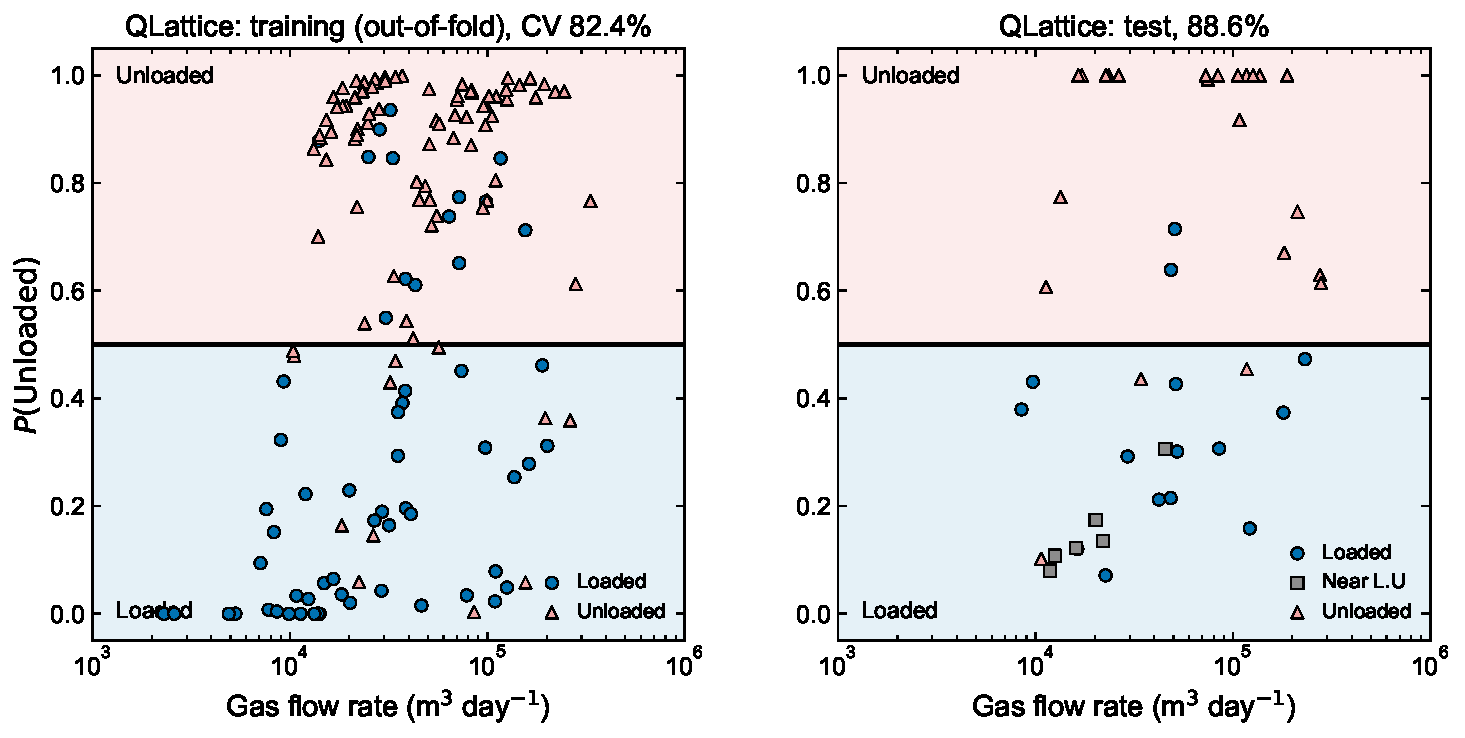
\includegraphics[width=0.85\linewidth]{Figures/qlattice_parity_updated.pdf}
    \caption{\al{Predicted probability of the unloaded class from the QLattice model at the observed gas rate, for the training wells (left, out-of-fold predictions from 5-fold cross-validation) and the test wells (right). Wells above 0.5 are predicted unloaded. Colors and symbols as in Figure \ref{M-class_acc} of the main text.}}
    \label{fig:si_qlattice}
\end{figure}

\section{\al{TabPFN}}
\al{The TabPFN classifier (\texttt{tabpfn} 6.0.6, default settings, CPU) was given $\ln Q_{\text{operating}}$ and the ten well features. Wells were classified from the predicted probability of the unloaded class at the measured operating rate. To test whether an implied critical rate exists, the operating rate of each test well was swept over 241 logarithmically spaced values between $10^{-6}$ and $10^{6}$ times its measured rate, with all other features fixed. The predicted probability crossed 0.5 for only 15 of the 44 test wells; for the remaining 29 it stayed on one side of 0.5 over the entire range, so no implied critical rate exists. The same sweep applied to the QLattice model found no crossing for 13 test wells, 12 of which have a non-positive argument of the logarithm in eq. (\ref{M-eq:qlattice_new}). Figure \ref{fig:si_tabpfn} shows the predicted probabilities.}

\begin{figure}[H]
    \centering
    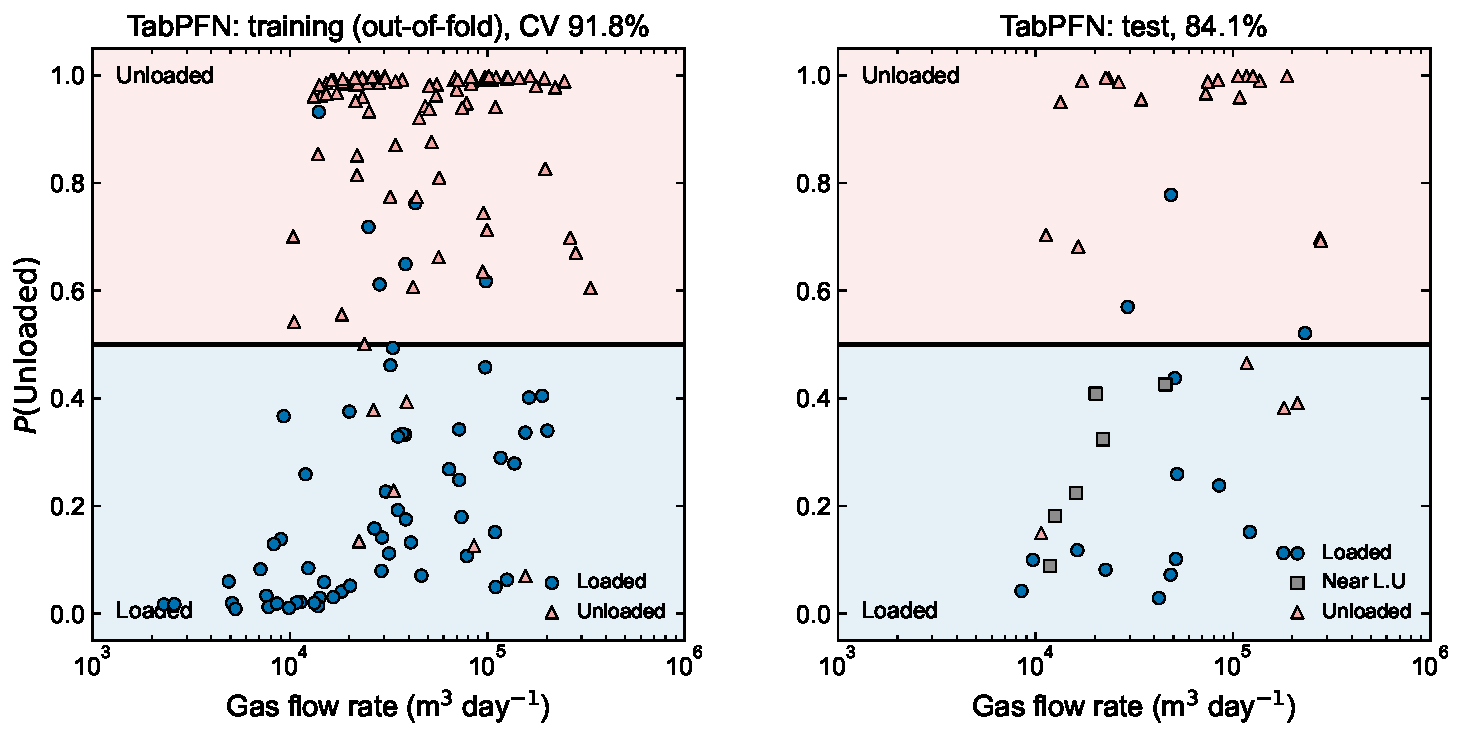
\includegraphics[width=0.85\linewidth]{Figures/tabpfn_parity_updated.pdf}
    \caption{\al{Predicted probability of the unloaded class from the TabPFN model at the observed gas rate, for the training wells (left, out-of-fold) and the test wells (right). Wells above 0.5 are predicted unloaded.}}
    \label{fig:si_tabpfn}
\end{figure}

\section{Prediction performance using different theories}

This section presents the performance of models developed based on each individual theory without combining them. \al{The droplet-only model (LDM) and film-only model (LFM) were fitted within the same framework as the DFM (same loss, data split, classification rule, and residual correction) by fixing $\alpha = 0$ (LDM) or $\alpha = 1$ (LFM) in eq. (\ref{M-eq:combined}) of the main text (Table \ref{tab:si_baselines}; Figures \ref{droplet_only} and \ref{film_only}).}

\begin{table}[H]
\centering
\caption{\al{Classification accuracy (\%) of the single-mechanism models and the DFM. CV: 5-fold cross-validation on the 148 training wells (mean $\pm$ standard deviation). Test: the 44 test wells, with the six near-loaded wells counted as loaded.}}
\label{tab:si_baselines}
\begin{tabular}{lcc}
\toprule
Model & CV & Test \\
\midrule
LDM & 85.1 $\pm$ 3.6 & 88.6 \\
LFM & 81.1 $\pm$ 4.6 & 86.4 \\
DFM & 85.8 $\pm$ 3.5 & 90.9 \\
\bottomrule
\end{tabular}
\end{table}

\al{Because the fitted DFM mixing parameter is small ($\alpha = 0.0025$), the DFM is close to droplet-only, and the LDM residual is nearly identical to that of the DFM (Tables \ref{tab:si_resid_single} and \ref{tab:si_residual}). The LFM residual is much larger, with an intercept of 6.6 and a strong negative weight on $\cos\theta$, which compensates for the vanishing film critical rate in horizontal wells.}

\begin{table}[H]
\centering
\caption{\al{Fitted residual corrections of the single-mechanism models ($\lambda = 0.1$, training set). Weights refer to standardized features; a positive weight increases the critical rate.}}
\label{tab:si_resid_single}
\begin{tabular}{lrr}
\toprule
Term & LDM & LFM \\
\midrule
Intercept $b$ & $-0.035$ & 6.616 \\
Logistic slope $k$ & 1.070 & 0.861 \\
$\ln \delta_{\text{crit}}$ & 2.369 & 3.878 \\
$\ln D$ & 2.328 & 4.081 \\
$\sin\theta$ & 0.971 & $-0.563$ \\
$\cos\theta$ & 0.266 & $-5.884$ \\
$\ln \rho_l$ & 0.733 & $-1.824$ \\
$\ln (P/T)$ & 0.612 & 1.872 \\
$\ln z$ & 0.330 & $-0.635$ \\
$\ln f_i$ & 0.251 & 0.137 \\
$\ln \rho_g$ & $-0.079$ & $-0.127$ \\
\bottomrule
\end{tabular}
\end{table}

\subsection{Droplet Only}
For the droplet-only case, the \al{physics part of the} critical rate \al{obtained on the training set} is:

\begin{equation}
\al{Q_{\mathrm{cr}} = 1.54\times 10^{7} \cdot 
\sqrt{ \frac{\left| \sin(2.612\,\theta) \right|^{2.563} \, |\rho_l - \rho_g|^{0.000}}{\rho_g^2} 
\cdot \frac{P}{T z} }}
\end{equation}
\al{The fitted density-difference exponent is effectively zero. The critical rate of the LDM with residual is this expression multiplied by $\exp(b + \mathbf{w}^\top \tilde{\mathbf{x}})$ with the LDM values in Table \ref{tab:si_resid_single}.}
\begin{figure}[H]
    \centering
    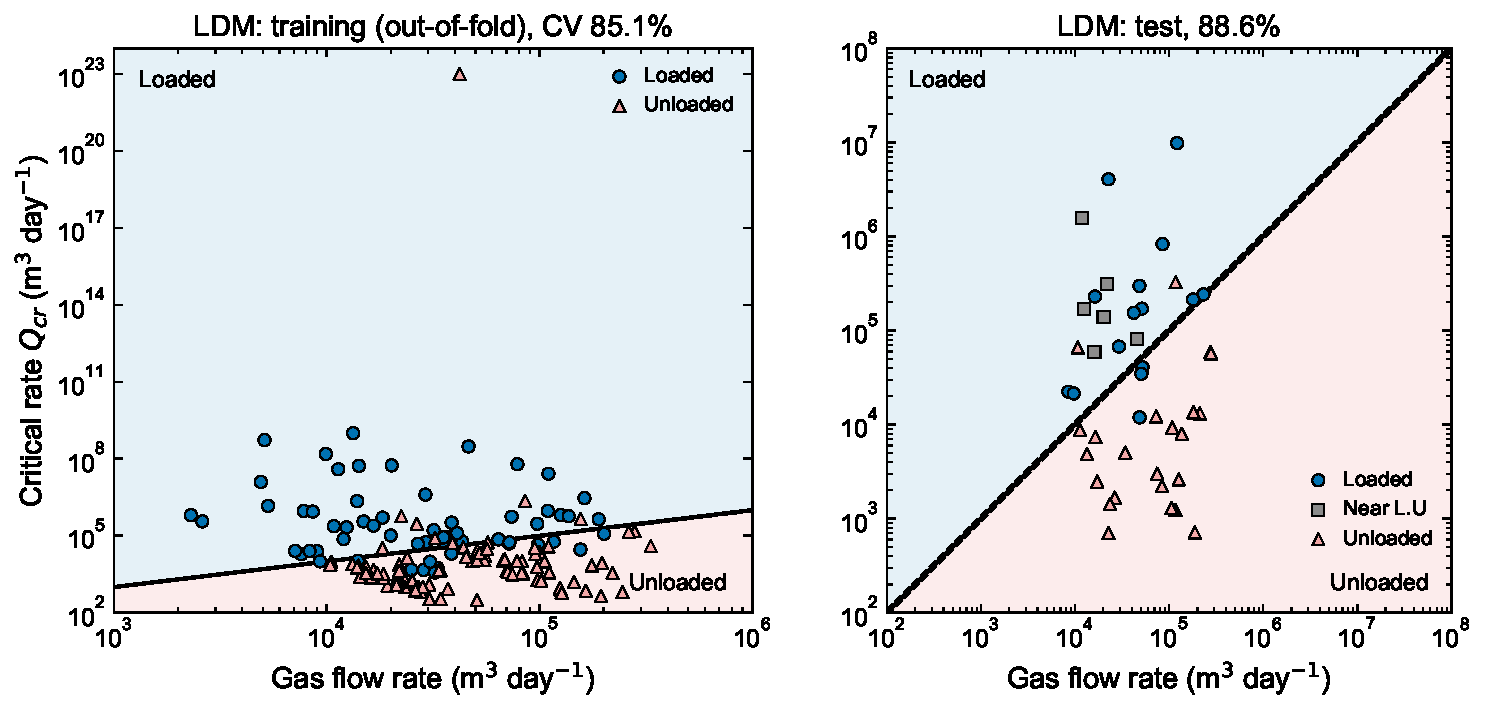
\includegraphics[width=0.85\linewidth]{Figures/ldm_parity_updated.pdf}
    \caption{\al{Critical rate of the droplet-only model (LDM, with residual) versus the observed gas rate for the training wells (left, out-of-fold) and the test wells (right). All wells lie within the axes; the training panel uses wider axes because a few out-of-fold critical rates are very large.}}
    \label{droplet_only}
\end{figure}

\subsection{Film Only}
\label{sec:fil_only-performance}
For the film-only case, The force balance for the entire fluid is expressed as:
\begin{equation}
- \frac{dp}{dx} \frac{\pi D^2}{4} + \tau_w \pi D - \left[ \rho_l (1 - \beta) + \rho_g \beta \right] \frac{\pi D^2}{4} g \cos{\theta} = 0
\label{eq:ODE1}
\end{equation}
\noindent where \( p \) = pressure (MPa); \( x \) = direction of flow; \( D \) = diameter of tubular pipe (m); \( \tau_w \) = liquid-wall shear stress (MPa); \( \rho_l \) and \( \rho_g \) = densities of liquid and gas respectively (kg/m³); \( \beta \) = volumetric gas concentration; \( g \) = acceleration due to gravity (m/s²); \( \theta \) = deviation angle in degrees. The force balance for the gas core at the center region of the wellbore is written as:
\begin{equation}
- \frac{dp}{dx} \frac{\pi D^2}{4} \beta - \tau_i \pi D \sqrt{\beta} - \rho_g \beta \frac{\pi D^2}{4} g \cos{\theta} = 0
\label{eq:ODE2}
\end{equation}
where \( \tau_i \) = liquid-gas interfacial shear stress (MPa). Dividing through Eq. (\ref{eq:ODE2}) by \( \beta \) and adopting the combined momentum Eqs. (\ref{eq:ODE1}) and (\ref{eq:ODE2}) for annular flow pattern gives:
\begin{equation}
\frac{4 \tau_w}{D} + \frac{4 \tau_i}{D \sqrt{\beta}} - (\rho_l - \rho_g) g (1 - \beta) \cos{\theta} = 0
\label{eq:ANNULAR}
\end{equation}
Taking into account the liquid wall shear stress, the liquid-gas interfacial friction factor, and the flow coefficients established by Taitler and Dukler\cite{https://doi.org/10.1002/aic.690220105}:
\begin{equation}
\tau_w = C_w \left( \frac{D V_l \rho_l}{\mu_l} \right)^{-a} \frac{\rho_l V_l^2}{2}
\label{eq:TW}
\end{equation}
\begin{equation}
V_l = \frac{V_{sl}}{(1 - \beta)}
\label{eq:VSL}
\end{equation}
Substituting Eq. (\ref{eq:TW} and \ref{eq:VSL}) into and rearrangement gives Eq. (\ref{eq:ANNULAR}) :
\begin{equation}
\tau_i = \frac{D \sqrt{\beta}}{4} (\rho_l - \rho_g) g (1 - \beta) \cos{\theta} - C_w \sqrt{\beta} \left( \frac{D V_{sl} \rho_l}{\mu_l (1 - \beta)} \right)^{-a} \frac{\rho_l V_{sl}^2}{(1 - \beta)^2}
\label{eq:reArr}
\end{equation}
where \( \tau_w \) = Liquid-wall shear stress, \( f_w \) = liquid interfacial friction factor, and \( V_{sl} \) = superficial liquid velocity, m/s\(^2\). Introduction of non-dimensionality:
\begin{equation}
1 - \beta = \frac{4 \delta}{D} (1 - \frac{\delta}{D})
\end{equation}
\begin{equation}
\bar{\delta} = \frac{\delta}{D}
\end{equation}
where \( \delta \) = film thickness (m); \( \bar{\delta} \) = dimensionless film thickness. Substituting \( \beta \) from the dimensionless equation to Eq (\ref{eq:reArr})\cite{OKORO20192443} :
\begin{equation}
\tau_i = (\rho_l - \rho_g) g D \cos{\theta} (1 - 2 \bar{\delta}) (\bar{\delta} - \bar{\delta}^2) - \frac{1}{2} C_w \rho_l \left( \frac{D \rho_l}{\mu_l} \right)^{-a} V_{sl}^{2 - a} \left( \frac{1}{4 \bar{\delta} - 4 \bar{\delta}^2} \right)^{2 - a} (1 - 2 \bar{\delta})
\label{eq:reArr1}
\end{equation}
representation of the liquid gas interfacial shear stress given as:
\begin{equation}
\tau_i = f_i \frac{\rho_g V_{sg}^2}{2 (1 - 2 \bar{\delta})^4}
\label{eq:reArr2}
\end{equation}
Combining equation (\ref{eq:reArr1}) and equation (\ref{eq:reArr2}), making ${V_g}$ subject of the formula and applying the Shi \cite{shi2016} assumption on film balance gives the equation \ref{eq:film_si} which is the expression gotten by Okoro \textit{et al}.\cite{OKORO20192443}, to address issues with non-idealities in the film topography we introduced a simple correction factor $\mathrm{C}_{f1}$:
\begin{equation}
U_{{\mathrm{film,\,crit}}} = \mathrm{C}_{f_1} \, \sqrt{\frac{2 \, g \, \delta \, (1 - 3 \bar{\delta} + 3 \bar{\delta}^2) \, (\rho_l - \rho_g) \, \cos \theta}{f_i \, \rho_g}},
\label{eq:film_si}
\end{equation}

The mathematical expression for the \al{physics part of the} critical rate for the film only after regression is defined below\al{; the LFM with residual multiplies it by $\exp(b + \mathbf{w}^\top \tilde{\mathbf{x}})$ with the LFM values in Table \ref{tab:si_resid_single}}:

\begin{equation}
Q_{\text{cr}} = \al{29.2} \cdot 
\sqrt{ \left( 
\frac{
2g D \left( 1 - 3 \frac{D}{\delta} + \al{4} \left( \frac{D}{\delta} \right)^2 \right) (\rho_L - \rho_G) \cos(\theta)
}{
f \cdot \rho_G
} 
\right) 
\cdot \left( \frac{P}{Tz} \right)}
\end{equation}
\mz{[Note for coauthors: this fitted expression is written as implemented in the code, which differs from eq. (\ref{eq:film_si}): the code uses $D$ instead of $\delta$ in the prefactor, $D/\delta$ instead of $\bar\delta = \delta/D$, and a coefficient of 4 instead of 3 on the quadratic term. In addition, the code takes the square root of $(\alpha U_{\text{film}} + (1-\alpha) U_{\text{droplet}})\,P/(zT)$ rather than using eq. (\ref{M-eq:combined2}) of the main text. Please confirm which form is intended before submission.]}

\begin{figure}[H]
    \centering
    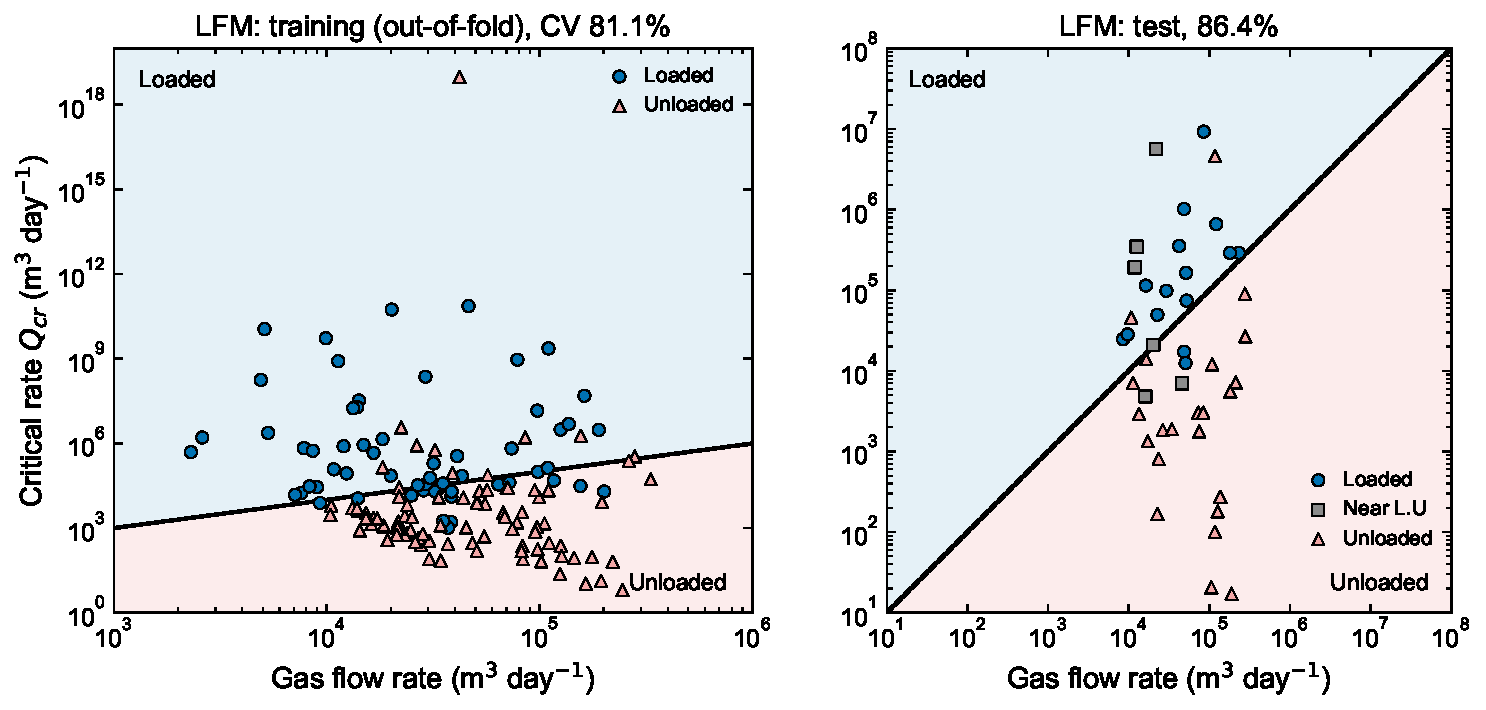
\includegraphics[width=0.85\linewidth]{Figures/lfm_parity_updated.pdf}
    \caption{\al{Critical rate of the film-only model (LFM, with residual) versus the observed gas rate for the training wells (left, out-of-fold) and the test wells (right). All wells lie within the axes; the training panel uses wider axes because a few out-of-fold critical rates are very large.}}
    \label{film_only}
\end{figure}

\section{\al{DFM model}}

\subsection*{\al{Physics parameters}}
\al{The physics parameters of the DFM were estimated with differential evolution (SciPy, 200 iterations, population size 15, seed 42) by minimizing eq. (\ref{eq:si_loss}) with $k = 4$. A single global mixing parameter $\alpha = \sigma(a)$ was used, where $\sigma$ is the logistic function. The fitted values are listed in Table \ref{tab:si_dfm_params}. Two parameters, the film scale $C_{f_1}$ and the logit $a$ of $\alpha$, reached the lower bounds of their search ranges. Because only their product enters the critical rate, this indicates that the data favor a small film contribution overall. Refitting with widened bounds changed the size of the film share but not its dependence on deviation angle.}

\begin{table}[H]
\centering
\caption{\al{Fitted physics parameters of the DFM (training set). The droplet term is $|\sin(p_1 \theta)|^{p_2} |\rho_l - \rho_g|^{p_4} / \rho_g^2$, and $C_{f_2}$ is the overall prefactor of the critical rate.}}
\label{tab:si_dfm_params}
\begin{tabular}{lll}
\toprule
Parameter & Value & Note \\
\midrule
$\ln C_{f_2}$ & 9.757 & overall prefactor \\
$p_4$ (density exponent) & 1.962 & \\
$p_2$ (angle exponent) & 1.302 & \\
$\ln C_{f_1}^2$ & $-10.0$ & lower bound \\
$p_1$ (angle multiplier) & 2.860 & \\
$a$, with $\alpha = \sigma(a)$ & $-6.0$ ($\alpha = 0.0025$) & lower bound \\
\bottomrule
\end{tabular}
\end{table}

\subsection*{\al{Residual correction}}
\al{The residual correction, eq. (\ref{M-eq:residual}) of the main text, was fitted with L-BFGS-B (SciPy) by minimizing eq. (\ref{eq:si_loss}) with $m_i = \ln Q_{\text{operating},i} - \ln Q_{\text{combined,crit},i} - b - \mathbf{w}^\top\tilde{\mathbf{x}}_i$, a learned slope $k$, and an L2 penalty $\lambda \lVert \mathbf{w} \rVert^2 / N$. The features $\tilde{\mathbf{x}}$ were standardized with the training-set mean and standard deviation. The penalty strength was selected by 5-fold CV on the training set (Table \ref{tab:si_lambda}). The fitted residual parameters are listed in Table \ref{tab:si_residual}.}

\begin{table}[H]
\centering
\caption{\al{5-fold CV accuracy of the DFM for different strengths $\lambda$ of the L2 penalty on the residual weights.}}
\label{tab:si_lambda}
\begin{tabular}{lcccccc}
\toprule
$\lambda$ & 0.03 & 0.1 & 0.3 & 1 & 3 & 10 \\
\midrule
CV accuracy (\%) & 85.1 & \textbf{85.8} & 83.7 & 83.0 & 80.4 & 79.0 \\
\bottomrule
\end{tabular}
\end{table}

\begin{table}[H]
\centering
\caption{\al{Fitted residual correction of the DFM ($\lambda = 0.1$). Weights refer to standardized features; a positive weight increases the critical rate.}}
\label{tab:si_residual}
\begin{tabular}{lr}
\toprule
Term & Value \\
\midrule
Intercept $b$ & $-0.005$ \\
Logistic slope $k$ & 1.109 \\
$\ln \delta_{\text{crit}}$ & 2.286 \\
$\ln D$ & 2.245 \\
$\sin\theta$ & 1.050 \\
$\ln \rho_l$ & 0.589 \\
$\ln (P/T)$ & 0.563 \\
$\ln z$ & 0.349 \\
$\cos\theta$ & 0.329 \\
$\ln f_i$ & 0.290 \\
$\ln \rho_g$ & $-0.073$ \\
\bottomrule
\end{tabular}
\end{table}

\al{The learned slope $k \approx 1.1$ implies a gradual transition between the classes: the predicted probability of the unloaded class changes from 0.25 to 0.75 over a factor of about 7 in $Q_{\text{operating}}/\hat Q_{\text{cr}}$. This reflects the substantial overlap of loaded and unloaded wells in the data. Consequently, the DFM critical rates are well constrained in sign relative to the operating rate, but their magnitude carries considerable uncertainty. In preliminary tests, fixing $k = 4$ kept the critical rates closer to the operating rates but reduced the CV accuracy by approximately 4--5 percentage points.}

\begin{figure}[H]
    \centering
    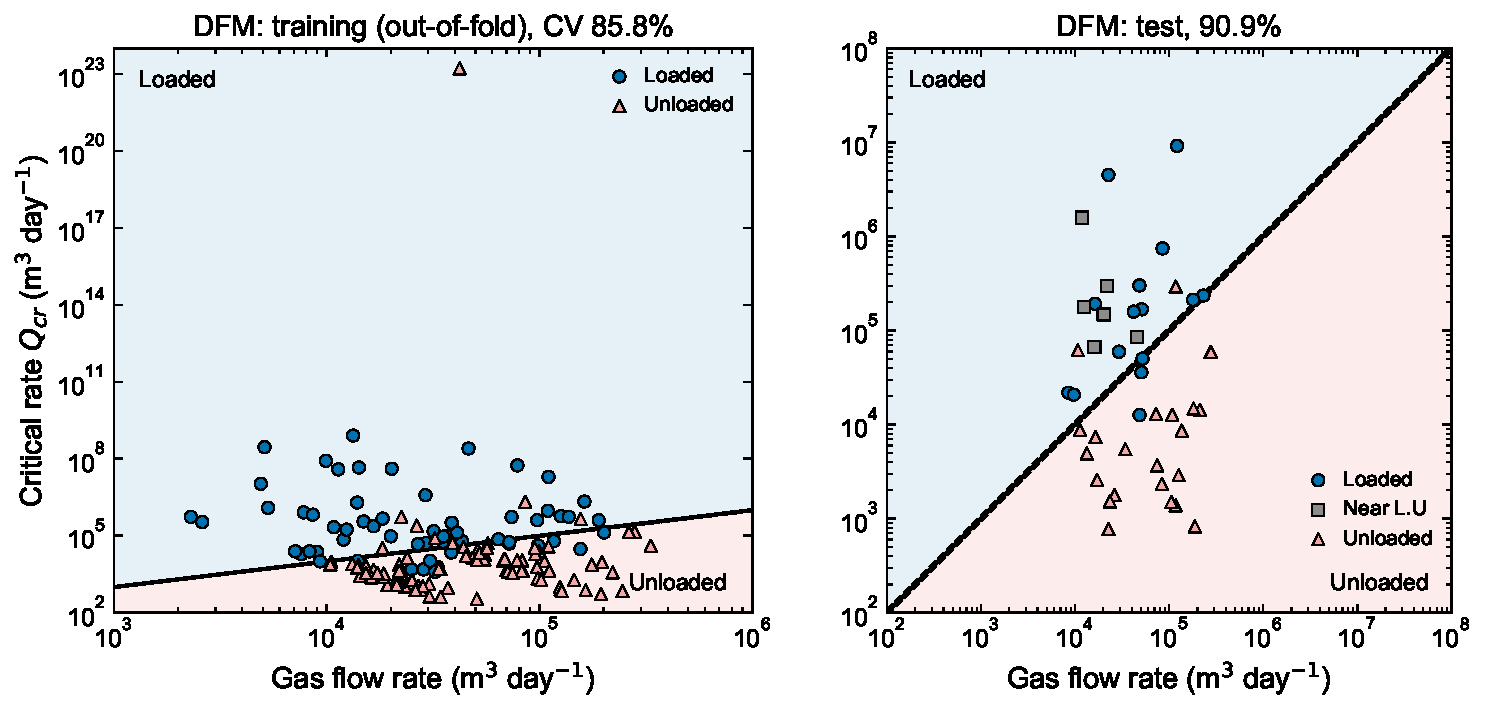
\includegraphics[width=0.85\linewidth]{Figures/dfm_parity_updated.pdf}
    \caption{\al{Critical rate of the DFM versus the observed gas rate for the training wells (left, out-of-fold) and the test wells (right). All wells lie within the axes; the training panel uses wider axes because a few out-of-fold critical rates are very large.}}
    \label{fig:si_dfm}
\end{figure}

\begin{figure}[H]
    \centering
    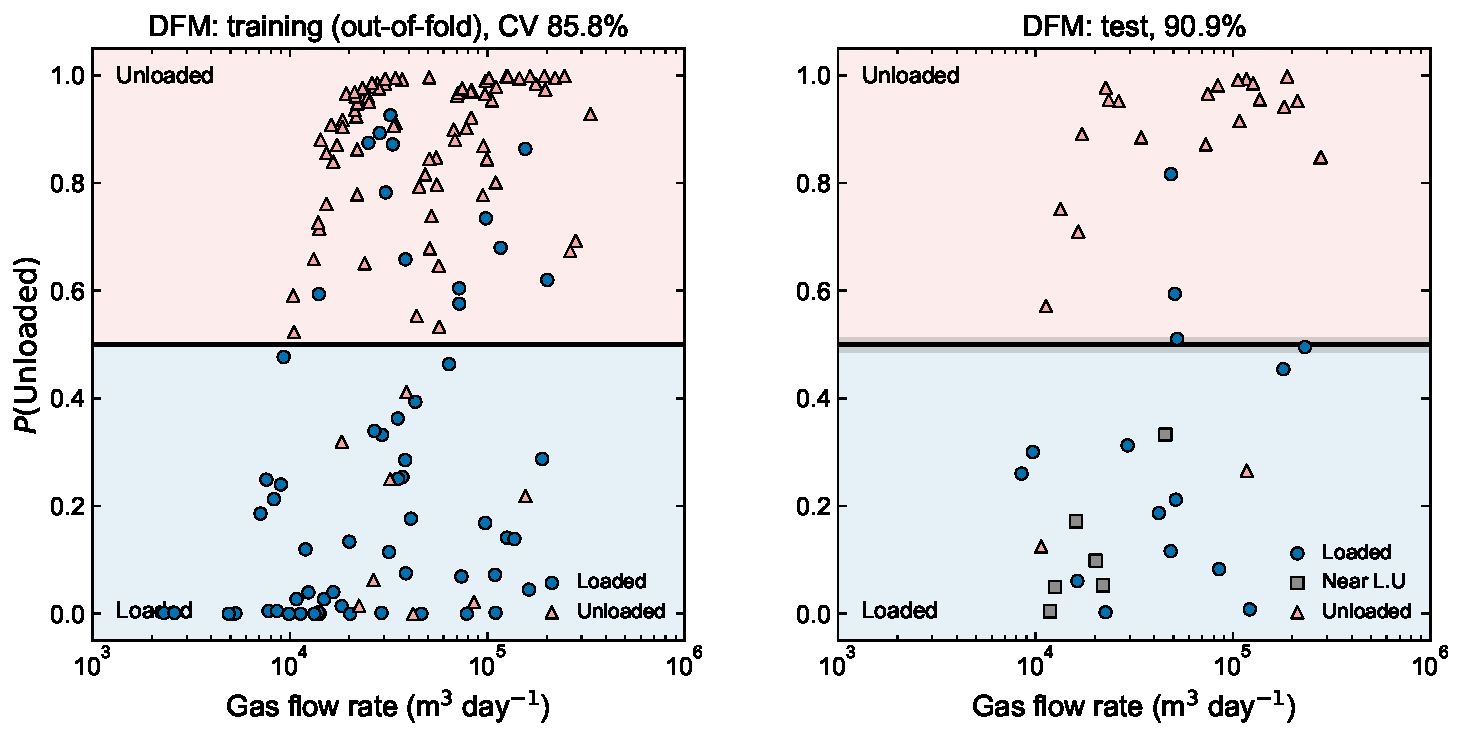
\includegraphics[width=0.85\linewidth]{Figures/dfm_probability_updated.pdf}
    \caption{\al{Predicted probability of the unloaded class from the DFM, $\sigma(k \ln(Q_{\text{operating}}/\hat Q_{\text{cr}}))$, at the observed gas rate, for the training wells (left, out-of-fold; each fold uses its own learned slope, $k = 1.13$--$1.31$) and the test wells (right, $k = 1.11$). Wells above 0.5 are predicted unloaded; the thin gray strip in the test panel marks the $\pm$5\% near-loaded band. This is the same quantity as shown for QLattice and TabPFN in Figures \ref{fig:si_qlattice} and \ref{fig:si_tabpfn}.}}
    \label{fig:si_dfm_prob}
\end{figure}

\section{\al{Additional classification diagnostics}}

\begin{figure}[H]
    \centering
    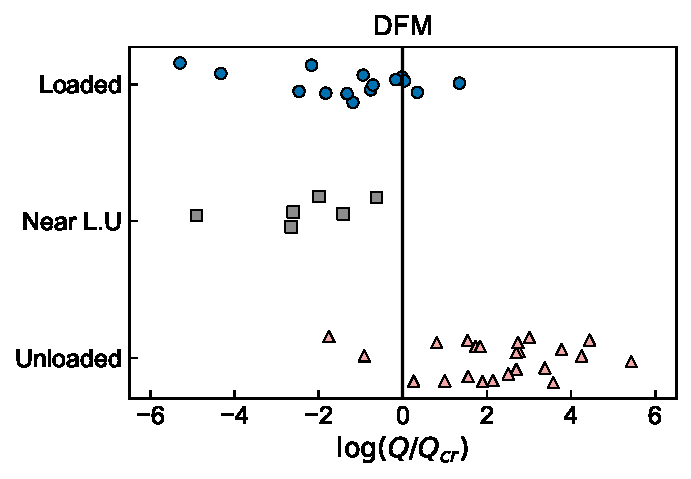
\includegraphics[width=0.55\linewidth]{Figures/margin_by_status_updated.pdf}
    \caption{\al{Classification margin $\ln(Q_{\text{operating}}/\hat Q_{\text{cr}})$ of the DFM for the test wells, grouped by true status. Wells to the right of zero are predicted unloaded and wells to the left loaded; the gray strip marks the near-loaded band ($\pm 0.05$). All six near-loaded wells fall well to the left of the band. QLattice and TabPFN are not shown because their implied critical rate does not exist for many wells (Figures \ref{fig:si_qlattice} and \ref{fig:si_tabpfn} show their predicted probabilities instead).}}
    \label{fig:si_margin}
\end{figure}

\begin{figure}[H]
    \centering
    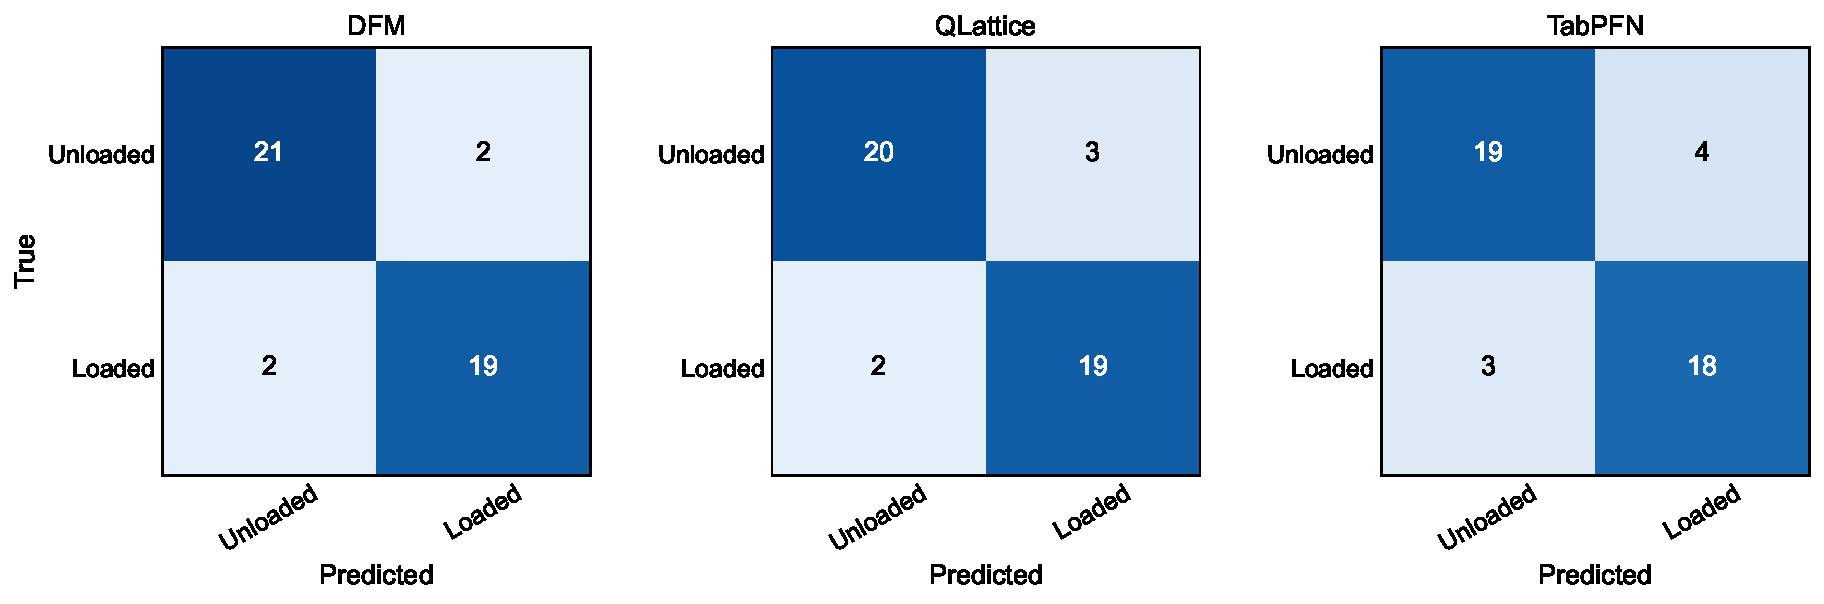
\includegraphics[width=0.95\linewidth]{Figures/confusion_matrices_updated.pdf}
    \caption{\al{Confusion matrices of the DFM, QLattice, and TabPFN models on the 44 test wells.}}
    \label{fig:si_confusion}
\end{figure}

\al{Because the true critical rate is not measured, regression metrics (e.g., RMSE or $R^2$ against a reference critical rate) are not meaningful for these models and are not reported; all performance measures are classification accuracies.}

\bibliography{sn-bibliography}

\end{document}
